\subsection{Les courbes obtenues}

Voici l'exemple d'une courbe obtenue (courbe 1, 99$^{eme}$ simulation de monte-carlo) :

\begin{figure}[H]
	\centering
	\textbf{Données simulées}

	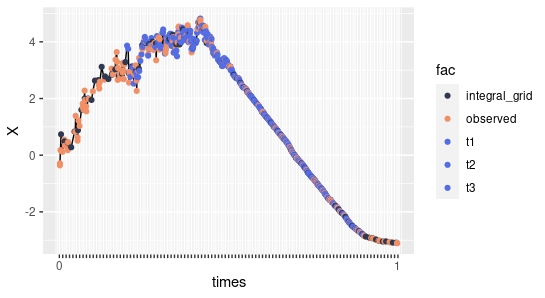
\includegraphics[width=0.48\textwidth]{Images/simul/all.jpeg}
	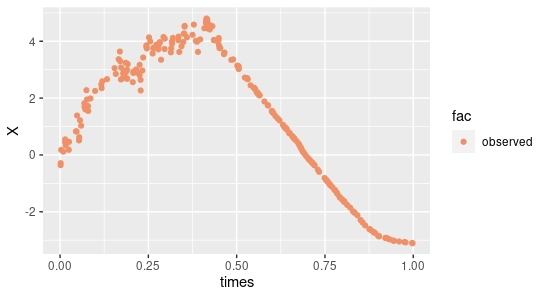
\includegraphics[width=0.48\textwidth]{Images/simul/observed.jpeg}

	\textbf{Lissage des données}

	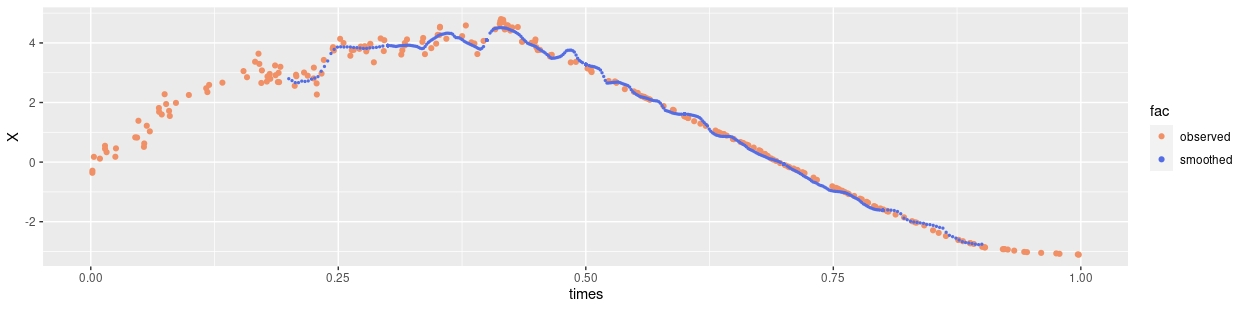
\includegraphics[width=0.96\textwidth]{Images/simul/smoothed.jpeg}
	\caption{Visualisation des données générées : $\lambda = 255, N = 200,$ 30 valeurs de $\Delta$}
\end{figure}


\subsection{Pré-Lissage}

Le pré-lissage des courbes a été fait en utilisant un lissage non paramétrique à noyaux\footnote{Il était aussi prévu d'effectuer un pré-lissage spline et à ondelettes mais le temps a eu raison de ce projet}. Comme mentionné dans la section \ref{eq:h_cross_noyau_pre}, chaque courbe est lissée en utilisant une fenêtre par validation croisée avec la grille $\mathcal H= \{ 0.01 \dots 0.2 \}_{50}$ avec pour métrique une estimation du risque quadratique $\esperance{|\widehat Y_{(-i)} - Y|^2}$. On ne regarde pas de fenêtre au delà de $\Delta = 0.2$ car il serait difficile de justifier pour l'estimation de la régularité que l'on lisse en regardant plus de $20$\% du support alors que la régularité évolue sur l'ensemble de l'intervalle.

L'obtention de la fenêtre de lissage a été réalisée en réalisant une validation croisée sur une grille de fenêtre étalées sur une échelle de puissance entre $h_{min} = 2 / \widehat \lambda$ et $h_{max} = 1 / \widehat \lambda^{1/3}$.

\begin{align*}
	                                                 & \mathcal H = \bigl\{ h_k, \, k \in \llbracket 1, K \rrbracket \bigr\}
	\\
	\forall k \in \llbracket 1, K \rrbracket, \qquad & h_k = h_{min} e^{ - a \cdot k }
	\\
	\text{avec } \qquad                              & a = \frac{\log \left( h_{max} \right) - \log(h_{min})}{K}
	\\
	\textsf{de valeur max} \qquad                    & h_K = h_{max} = h_{min} e^{ - a \cdot K }
	\\
	\text{et } \qquad                                & K = 30
\end{align*}

Cela est dû au fait que $h^*_{\mathcal R_{\textsf{quadr}}} = \grandop{ \lambda^{- \frac 1 {1 + 2H_t}} }$ avec $0<H_t<1$, comme vu dans la section \ref{sec:regloc-prelissage}. De plus, on souhaite que dans notre fenêtre de lissage, en moyenne, se trouvent 2 points au minimum. 

